%%%%%%%%%%%%%%%%%%%%%%%%%%%%%%%%%%%%%%%
% Project N°5 for ITY
% Author: Michal Ormos
% Date:   21.4.2015
%%%%%%%%%%%%%%%%%%%%%%%%%%%%%%%%%%%%%%%

\documentclass[fyma2,pdf,final,hyperref={unicode},hyperref={pdfpagelabels=false}]{beamer}[24.4.2015]
\usepackage[czech]{babel}
\usepackage[utf8]{inputenc}
\usetheme{Warsaw}
\usepackage{graphicx}
\usepackage{lmodern}
\usepackage{epstopdf}


\begin{document}

\title{Vývoj písma}  
\author{Michal Ormoš}
\date{\today}
\maketitle

\frame{\frametitle{Obsah}\tableofcontents} 


\section{Úvod} 
\subsection{Písmo}
\frame{\frametitle{Písmo} 
\begin{itemize}

\item Písmo vzniklo z prirodzenej potreby trvalejšieho zaznamenávania ľudskej reči a ďalšieho sprostredkovania myšlienok a udalostí v ich živote.
\item Na dejiny písma sa možno pozerať troma hlavnými spôsobmi:
\begin{enumerate}
\item možno sledovať, ako sa jednotlivé písma vyvíjali jedno z druhého (napríklad ktoré všetky písma sa vyvinuli z gréckeho písma)
\item možno sledovať, ako sa postupne vývojom menil typ písma nezávisle od jednotlivých písiem (napríklad ako prebiehal prechod od logografického písma k slabičnému)
\item a možno sledovať podrobnosti vývoja jednotlivých písem (napríklad vývoj čínskeho písma).
\end{enumerate}
\end{itemize}
}
\subsection{Vývoj písma z hľadiska vývojového stromu jednotlivých písiem}
\frame{\frametitle{Vývoj}
\begin{itemize}
  \item Európa a západná Ázia
  \item Ostatná Ázia
  \item Afrika
  \item Severná Amerika
  \item Stredná Amerika
\end{itemize}
}

\section{Rozdelenie}
\subsection{Podrobné rozdelenie}
\frame{\frametitle{Podrobné rozdelenie}

\begin{block}{Európa a západná Ázia:}
\begin{itemize}
  \item sumerské písmo
  \item protoelamské písmo
  \item krétske hieroglyfické písmo
\end{itemize}
\end{block}

\begin{exampleblock}{Ostatná Ázia:}
\begin{itemize}
  \item bráhmí
  \item tibetské písmo
  \item čínske písmo
\end{itemize}
\end{exampleblock}


\begin{alertblock}{Afrika:}
\begin{itemize}
  \item egyptské písmo
\end{itemize}
\end{alertblock}
}

\section{Príklady písma zo západnej Ázie, Afriky a Číny} 

\subsection{Sumerské písmo}
\frame{\frametitle{Sumerské písmo}
\begin{figure}
        \centering
            \scalebox{0.3}{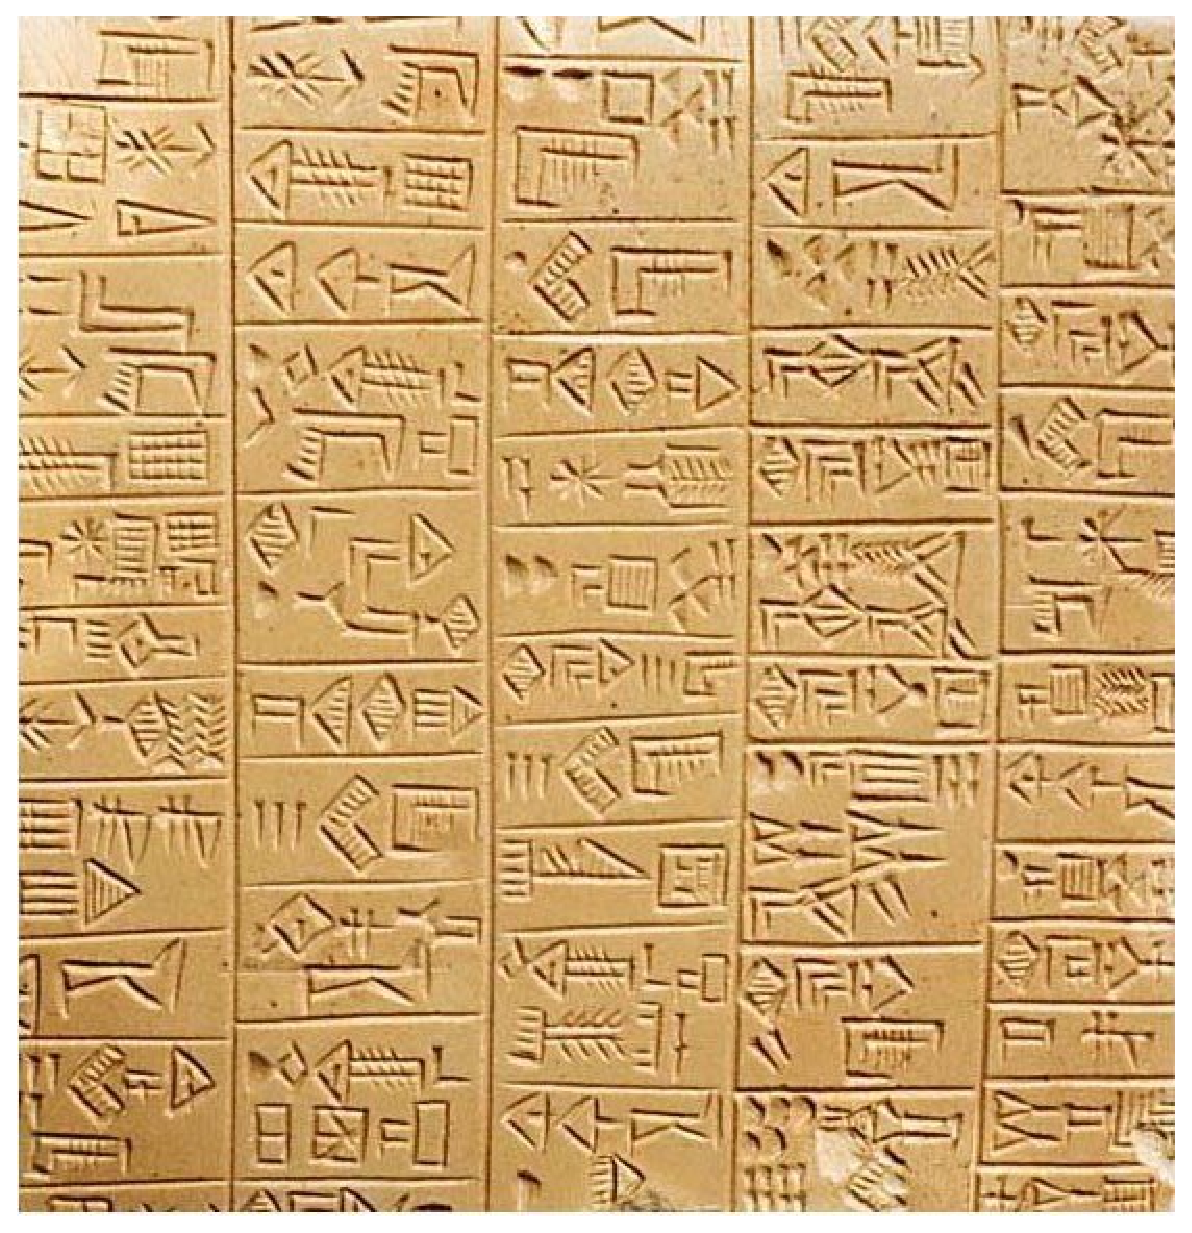
\includegraphics{sumerian_font.eps}}      
\caption{Príklad sumerského písma}
\label{pic:obr1}
\end{figure}
}

\subsection{Čínske písmo}
\frame{\frametitle{Čínske písmo}
\begin{figure}[h]
        \begin{center}
            \scalebox{0.4}{
\includegraphics{china_font.eps}}      
        \end{center}
\caption{Príklad čínskeho písma}
\label{pic:obr2}
\end{figure}
}

\subsection{Egyptské písmo}
\frame{\frametitle{Egyptské písmo}
\begin{figure}[h]
        \begin{center}
            \scalebox{0.2}{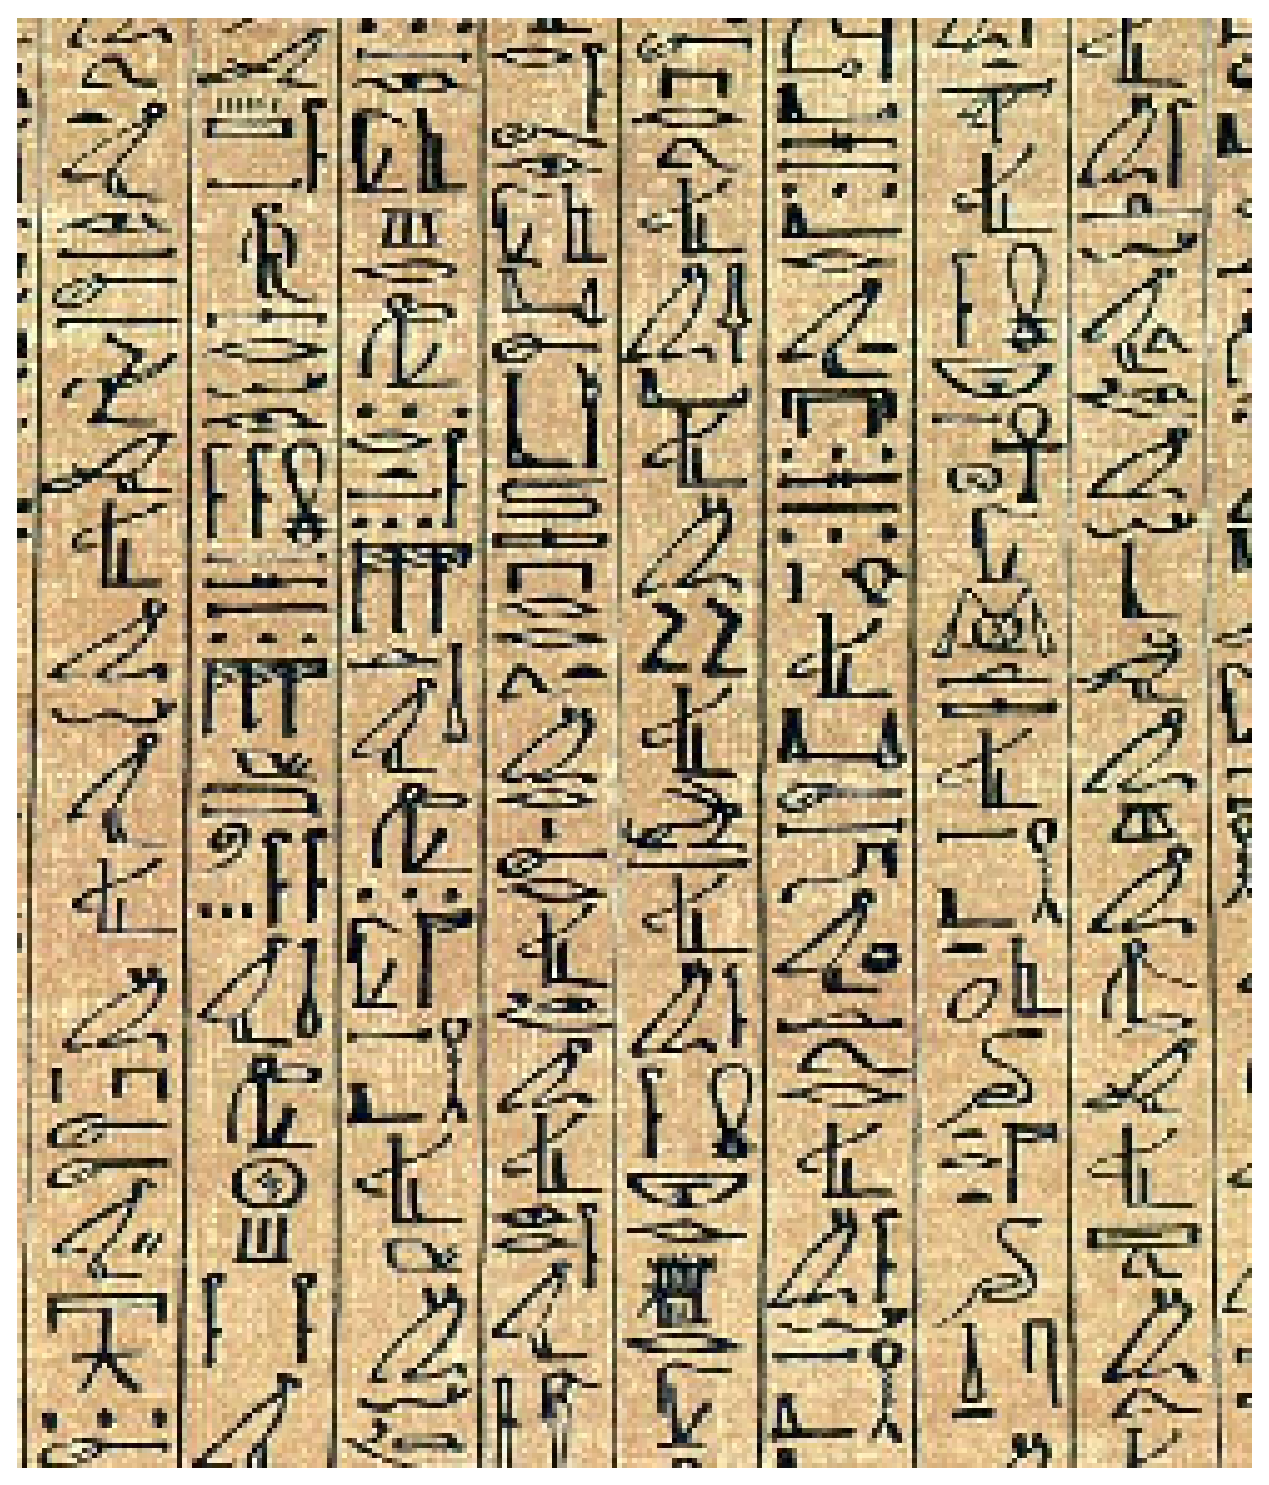
\includegraphics{egypt_font.eps}}      
        \end{center}
\caption{Príklad egyptského písma - hieroglyfy}
\label{pic:obr3}
\end{figure}
}

\end{document}
